Once upon a time the Conneaut Cable Advisory Board said they were
entering into discussions with Vimeo to shift their public access
channel off cable to streaming video. Great Wave Communications was
wanting to get out of the cable television business as it wasn't
profitable enough to them any more. That was in 2020 but I hadn't heard
anything further. Fast forward to 2022 and I finally found their
presence on Vimeo. Conneaut CAT-TV can be found at
\url{https://vimeo.com/user126359532}. Sadly it is mostly video on
demand rather than streaming.

There \emph{was} a PEG (public/education/government) channel on Charter
Spectrum's system in Ashtabula that was used historically by Ashtabula
Area City Schools. There was also one used by the Ashtabula campus of
Kent State University. It doesn't look like either are still
operational. Kent State Ashtabula transitioned over to using YouTube as
part of what appears to be a system-wide shift.

There aren't many video programming originators in Ashtbula County
outside churches and the local governments broadcasting video of their
meetings. The Conneaut Cable Advisory Board is the most general purpose
program originator that we have.

I would do a screen cap of the
\href{https://www.facebook.com/ashtabulacountyso/}{Facebook page for the
county sheriff's office} but frankly the level of ignorant comments by
residents are just embarassing. We should do better than this. This may
be somewhat indicative of why people leave this area \emph{and never
come back}.

\begin{figure}
\centering
\pandocbounded{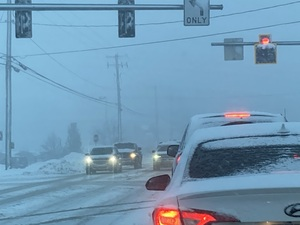
\includegraphics[keepaspectratio]{\%7B\%7Bsite.url\%7D\%7D/img/snowy-junction-20-and-11.jpg}}
\caption{Scaled shot of the intersection of United States Route 20 and
Ohio Route 11}
\end{figure}
